\section{System Architecture}

\label{sec:system}
\begin{figure*}
\centering
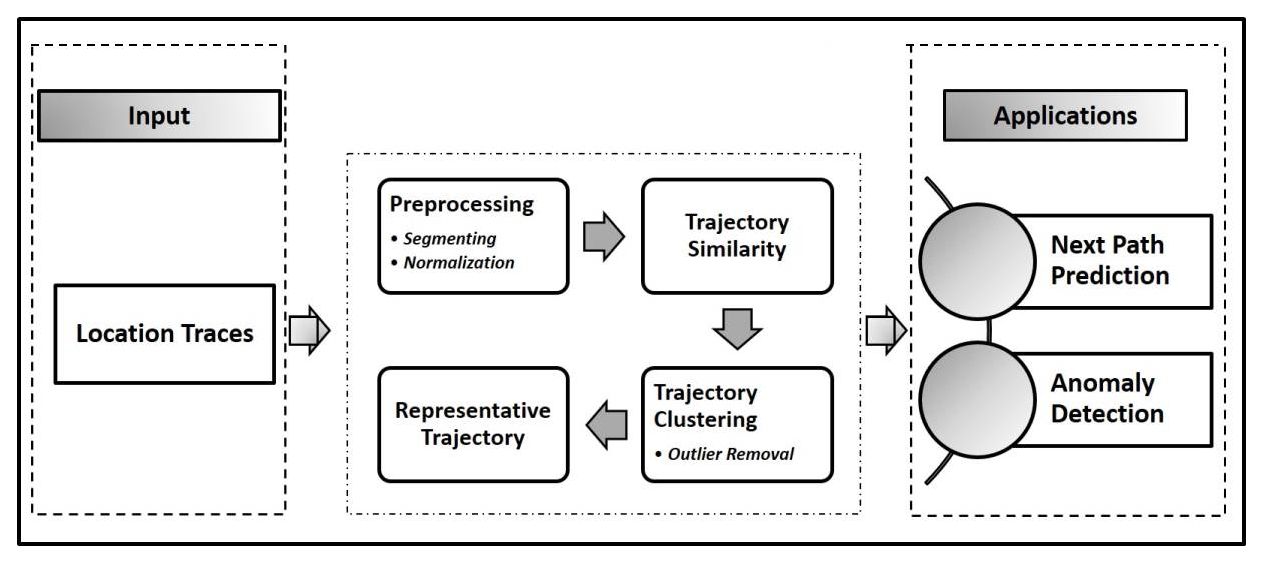
\includegraphics[scale=0.5]{figs/system_arch.eps}
\caption{Conceptual Architecture}
\label{fig:flow}
\end{figure*}

Figure \ref{fig:flow} describes the conceptual architecture of the Trajectory Summary Framework. The framework takes as inputs raw location traces, which are a collection of three tuples. The various aspects of the framework are described briefly.

\begin{itemize}
\item{\textbf{Trajectory Preprocessing:}}
This involves cleansing of the raw data and methods to extract meaningful trips or trajectories out of an input chunk, which is a collection of three tuples \emph{$\langle$ latitude, longitude, timestamp $\rangle$ }
\item{\textbf{Trajectory Similarity Analysis:}}
Attempts to define a similarity measure between two trajectories is the foundation of any kind of aggregation, or clustering. This module deals with defining a similarity which makes sense for human mobility. 
\item{\textbf{Trajectory Clustering:}}
This involves development of a trajectory clustering scheme. Given an input of trajectories, and a method which defines a similarity between two trajectories, the goal is to devise a clustering algorithm which outputs the final grouping of trajectories such that the final clusters define the \textit{Mobility Summary}  .
\item{\textbf{Representative Trajectory Computation:}}
Once the clusters are formed, a representative trajectory for each of the cluster needs to be computed, which would form the entire trajectory summarization.  
\item{\textbf{Applications of Mobility Summary:}}
The summarization module provides a compact abstraction for applications that query ``frequent-mobility''. Several use-cases can utilize the summary representation of the mobility pattern to provide insights. \textit{Next-path prediction} problem and \textit{Anomalous Movement Detection} are example applications that benefit from \trajSummary.
\end{itemize}

Each of the above modules is discussed in detail in the subsequent sections.


 




\begin{comment}
Various trajectory similarity metrics, which give an estimate of the trajectory distance, have been proposed. Standard LP-Norm and ERP have been shown to be metrics~\cite{Chen2004}, where as other heuristic functions (such as LCSS, DTW, EDR) are non-metrics~\cite{Vlachos2002,Yi1998,Chen2005}. We enhance LP-Norm to construct ``Weighted LP-Norm"', where more weights are given to the points closer to the origin and destination. This is based on the observation that, generally, a user's meaningful trip has an associated intention of commuting between two end-points (such as commuting to work or grocery shop visit).

\noindent\textbf{3. Trajectory Clustering}: 
In this module, hierarchical clustering is applied on the previously computed distance matrix. We choose hierarchical clustering because it gives us a way to store the trajectories of the user at various levels of granularity. Hierarchical clustering involves the computation of a dendrogram which describes how the trajectories are clustered throughout the various levels. We devise a function to cut the dendogram to form the right clusters based on earth-distance between the trajectory points of a cluster.
%The major obstacle is in finding the right number of clusters('k'). The most widely used method in literature to find the value of 'k' is to draw the plot of the number of clusters vs. Sum of Squared Errors within clusters, and finding the elbow point in the plot. However, in the case of human mobility, the clusters formed at the elbow point are very noisy. The heuristic we apply to come up with tighter, meaningful clusters is to go down the dendrogram, starting from the elbow point and reporting final clusters as and when the maximum point-wise earth-distance between all two trajectory pairs is less than a specified threshold $\delta$.

\noindent\textbf{4. Representative Trajectory:} 
We summarize the significant clusters by a representative trajectory for that cluster. We utilize the median trajectories~\cite{median1} because it provides parts of actual user traveled paths as representative trajectory.\\
\end{comment}